% !TeX root = construct.tex
\chapter{A Compass is Sufficient}\label{c.compass-only}

In 1797 the Italian mathematician Lorenzo Mascheroni proved that any construction carried out with a compass and straightedge can be carried out with the compass alone! In the twentieth century it was discovered that this theorem had been proved by the Danish mathematician Georg Mohr. The theorem is now called the Mohr-Mascheroni Theorem.

In this chapter I present a proof of the theorem based on a proof that appeared as problem 33 in \cite{dorrie1} and reworked by  Michael Woltermann \cite{dorrie2}.\footnote{I would like to thank him for giving me permission to use his work.} Additional proofs can be found in \cite{mm}, \cite{stopel}.

What does it mean to perform a construction with only a compass? The right diagram below shows the construction of an equilateral triangle using a straightedge and compass. How can we construct a triangle without the line segments $AB, AC,BC$? In fact, there is no need to \emph{see} the lines. A line is defined by two points, so it is sufficient to construct the points in order to obtain a construction equivalent to the one with a straightedge (left diagram):
\begin{center}
\begin{tikzpicture}[scale=0.6]
\coordinate (A) at (0,0);
\coordinate (B) at (4,0);
\path (A) node[below left] {$A$} -- (B) node[below right] {$B$};
\fill (A) circle[radius=3pt];
\fill (B) circle[radius=3pt];
\draw[name path=larc] (A) ++(-10:4cm) arc (-10:80:4cm);
\draw[name path=rarc] (B) ++(-170:4cm) arc (-170:-260:4cm);
\path [name intersections={of=larc and rarc,by={t}}];
\fill (t) node[above right,xshift=-2pt,yshift=3pt] {$C$} circle[radius=3pt];
\begin{scope}[xshift=10cm]
\coordinate (A) at (0,0);
\coordinate (B) at (4,0);
\draw (A) node[below left] {$A$} -- (B) node[below right] {$B$};
\fill (A) circle[radius=3pt];
\fill (B) circle[radius=3pt];
\draw[name path=larc] (A) ++(-10:4cm) arc (-10:80:4cm);
\draw[name path=rarc] (B) ++(-170:4cm) arc (-170:-260:4cm);
\path [name intersections={of=larc and rarc,by={t}}];
\fill (t) node[above right,xshift=-2pt,yshift=3pt] {$C$} circle[radius=3pt];
\draw (A) -- (t);
\draw (B) -- (t);
\end{scope}
\end{tikzpicture}
\end{center}
In the diagrams we will draw lines, but they are used only to understand the construction and the proof of its correctness. It is important that you convince yourself that the construction itself uses only a compass.

Every step of a construction with straightedge and compass consists of one of the following three operations:
\begin{itemize}
\item Finding the point of intersection of two straight lines.
\item Finding the point of intersection of a straight line and a circle.
\item Finding the point(s) of intersection of two circles.
\end{itemize}
It is clear that the third operation can be done with only a compass. We need to show that the first two operations can be done with a compass alone.

Notation:
\begin{itemize}
\item $C(O,A)$: the circle with center $O$ through point $A$.
\item $C(O,r)$: the circle with center $O$ and radius $r$.
\item $C(O,AB)$: the circle with center $O$ and radius the length of line segment $AB$.
\end{itemize}

First we will solve four preliminary problems (Sections~\ref{s.reflection}--\ref{s.three}) and then we show the construction for finding the intersection of two lines (Section~\ref{s.two-lines}) and that of a line and a circle (Section~\ref{s.line-circle}).

%%%%%%%%%%%%%%%%%%%%%%%%%%%%%%%%%%%%%%%%%%%%%%%%%%%%%%%%%%%%%%%

\section{Reflection of a point}\label{s.reflection}

\textbf{Given a line $AB$ and a point $C$ not on $AB$, it is possible to build a point $C'$ which is a reflection of $C$ about $AB$.} $C'$ is a \emph{reflection} about a line segment $AB$ if $AB$ (or the line containing $AB$ is the perpendicular bisector of the line $CC'$.

We build a circle centered on $A$ passing through $C$ and circle centered on $B$ passing through $C$. The intersection of the two circles is the point $C'$ which is the reflection of $C$.
\begin{center}
\begin{tikzpicture}[scale=.65]
\coordinate (A) at (0,0);
\coordinate (B) at (4,0);
\coordinate (C) at (2.5,1.5);
\draw[thick,dashed] ($(B)!2!(A)$) -- ($(A)!2!(B)$);
\fill (A) node[above left] {$A$} circle[radius=2pt];
\fill (B) node[above right] {$B$} circle[radius=2pt];
\fill (C) node[above,yshift=4pt] {$C$} circle[radius=2pt];
\node[draw,circle through=(C),name path=ac] at (A) {};
\node[draw,circle through=(C),name path=bc] at (B) {};
\path [name intersections={of=ac and bc,by={x1,Cp}}];
\fill (Cp) node[below,yshift=-4pt] {$C'$} circle[radius=2pt];
\draw (C) -- (Cp);
\draw[thick,dashed] (A) -- (C);
\draw[thick,dashed] (B) -- (C);
\draw[thick,dashed] (A) -- (Cp);
\draw[thick,dashed] (B) -- (Cp);
\end{tikzpicture}
\end{center}
\textbf{Proof:} $\triangle ABC \cong \triangle ABC'$ by SSS since $AC,AC'$ are radii of the same circle as are $BC,BC'$, and $AB$ is a common side. Therefore, $\angle CAB = \angle C'AB$ so $AB$ is the angle bisector of $\angle CAC'$. But $\triangle CAC'$ is an isosceles triangle and the angle bisector $AB$ is also the perpendicular bisector of the base of the triangle $CC'$. By definition $C'$ is the reflection of $C$ around $AB$.

%%%%%%%%%%%%%%%%%%%%%%%%%%%%%%%%%%%%%%%%%%%%%%%%%%%%%%%%%%%%%%%

\section{Construct a circle with a given radius}\label{s.circle}

\textbf{Given points $A,B,C$, construct$c(A,BC)$.}

Construct $c(A,B)$ and $c(B,A)$ and let $X$ and $Y$ be their points of intersection.

\begin{center}
\begin{tikzpicture}[scale=.55]
\coordinate (A) at (0,1.5);
\coordinate (B) at (0,-1.5);
\coordinate (C) at (1.5,-3);
\coordinate (Cp) at (1.5,3);
\fill (A) node[above] {$A$} circle[radius=3pt];
\fill (B) node[below] {$B$} circle[radius=3pt];
\fill (C) node[below] {$C$} circle[radius=3pt];
%\fill (Cp) node[above] {$C'$} circle[radius=3pt];
\node[draw,circle through=(B),name path=ab] at (A) {};
\node[draw,circle through=(A),name path=ba] at (B) {};
\path [name intersections={of=ab and ba,by={Y,X}}];
\fill (X) node[above right,xshift=4pt] {$X$} circle[radius=3pt];
\fill (Y) node[above left,xshift=-4pt] {$Y$} circle[radius=3pt];
\draw[thick,dashed] ($(X)!2.3!(Y)$) -- ($(Y)!2!(X)$);
\end{tikzpicture}
\vspace*{-6pt}
\end{center}
Construct $C'$, the reflection of $C$ about line $XY$ as described in Section~\ref{s.reflection}.

\begin{center}
\begin{tikzpicture}[scale=.45]
\coordinate (A) at (0,1.5);
\coordinate (B) at (0,-1.5);
\coordinate (C) at (1.5,-3);
\coordinate (Cp) at (1.5,3);
\fill (A) node[right] {$A$} circle[radius=3pt];
\fill (B) node[right] {$B$} circle[radius=3pt];
\fill (C) node[below,yshift=-2pt] {$C$} circle[radius=3pt];
\fill (Cp) node[above,xshift=2pt,yshift=2pt] {$C'$} circle[radius=3pt];
\node[circle through=(B),name path=ab] at (A) {};
\node[circle through=(A),name path=ba] at (B) {};
\path [name intersections={of=ab and ba,by={Y,X}}];
\fill (X) node[above right,xshift=4pt] {$X$} circle[radius=3pt];
\fill (Y) node[above left,xshift=-4pt] {$Y$} circle[radius=3pt];
\node[draw,circle through=(C)] at (X) {};
\node[draw,circle through=(C)] at (Y) {};
\draw[thick,dashed] ($(X)!2.3!(Y)$) -- ($(Y)!2!(X)$);
%\draw (X) -- (Y) -- (C) -- (X) -- (Cp) -- (Y);
\draw[thick,dashed] (C) -- (Cp);
\end{tikzpicture}
\vspace*{-6pt}
\end{center}

$c(A,C')$ is the desired circle.

\begin{center}
\begin{tikzpicture}[scale=.5]
\coordinate (A) at (0,1.5);
\coordinate (B) at (0,-1.5);
\coordinate (C) at (1.5,-3);
\coordinate (Cp) at (1.5,3);
\fill (A) node[above,yshift=2pt] {$A$} circle[radius=3pt];
\fill (B) node[below,yshift=-2pt] {$B$} circle[radius=3pt];
\fill (C) node[below,yshift=-2pt] {$C$} circle[radius=3pt];
\fill (Cp) node[above,yshift=2pt] {$C'$} circle[radius=3pt];
\node[circle through=(B),name path=ab] at (A) {};
\node[circle through=(A),name path=ba] at (B) {};
\path [name intersections={of=ab and ba,by={Y,X}}];
\fill (X) node[above right,xshift=4pt] {$X$} circle[radius=3pt];
\fill (Y) node[above left,xshift=-4pt] {$Y$} circle[radius=3pt];
\node[circle through=(C)] at (X) {};
\node[draw,circle through=(C)] at (Y) {};
\draw[thick,dashed] ($(X)!2.3!(Y)$) -- ($(Y)!2!(X)$);
\path[name path=xy] (X) -- (Y);
\node[draw,thick,circle through=(Cp)] at (A) {};
\draw[very thick] (A) -- (Cp);
\draw[very thick] (B) -- (C);
\draw[very thick,name path=abline] (A) -- (B);
\draw[very thick,name path=ccp] (C) -- (Cp);
\path [name intersections={of=xy and abline,by={D}}];
\path [name intersections={of=xy and ccp,by={E}}];
\fill (D) node[above left] {$D$} circle[radius=3pt];
\fill (E) node[below right] {$E$} circle[radius=3pt];
\draw[thick,dashed] (D) -- (Cp);
\draw[thick,dashed] (D) -- (C);
\end{tikzpicture}
\vspace*{-4pt}
\end{center}

\textbf{Proof:} $A$ is the reflection of $B$ around $XY$ (since $\triangle YAX\cong \triangle YBX$) and $C'$ is the reflection of $C$ around the $XY$. By definition, $XY$ is the perpendicular bisector of $CC'$ and $AB$, so $C'E=EC$, $AD=DB$ and $\angle DEC=\angle DEC'(=90^\circ)$. $\triangle DEC\cong\triangle DEC'$ by SAS, so $DC=DC'$ and $\angle ADC'=\angle BDC$ (they are complementary to $\angle EDC'$, $\angle EDC$). Therefore, $\triangle ADC'\cong\triangle BDC$ by ASA, so $AC'=BC$.

%%%%%%%%%%%%%%%%%%%%%%%%%%%%%%%%%%%%%%%%%%%%%%%%%%%%%%%%%%%%%%%

\section{Addition and subtraction of line segments}\label{s.add-subtract}

\textbf{Given line segment $PQ$ of length $a$ and line segment $RS$ of length $b$, it is possible to construct line segments $QT,QU$ such that $PUQT$ is a line segment, where the length of $PU$ is $a-b$ and the length of $PT$ is $a+b$.}
\begin{center}
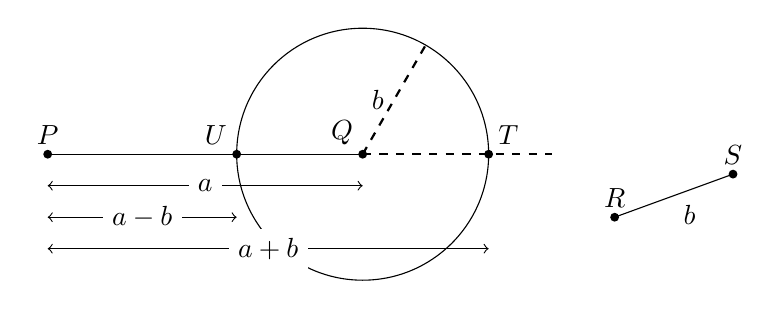
\begin{tikzpicture}[scale=.8]
\draw (0,0) -- (5,0);
\fill (0,0) node[above] {$P$} circle[radius=2pt];
\fill (5,0) node[above left] {$Q$} circle[radius=2pt];
\fill (3,0) node[above left] {$U$} circle[radius=2pt];
\fill (7,0) node[above right] {$T$} circle[radius=2pt];
\draw[thick,dashed] (5,0) -- (8,0);
\draw (5,0) circle[radius=2cm];
\draw[thick,dashed] (5,0) -- node[left] {$b$} ++(60:2cm);
\draw (9,-1) node[above] {$R$} -- node[below right] {$b$} ++(20:2cm) node[above] {$S$};
\fill (9,-1) circle[radius=2pt];
\fill (9,-1) ++(20:2cm) circle[radius=2pt];
\draw[<->] (0,-.5) -- node[fill=white] {$a$} (5,-.5);
\draw[<->] (0,-1) -- node[fill=white] {$a-b$} (3,-1);
\draw[<->] (0,-1.5) -- node[fill=white] {$a+b$} (7,-1.5);
\end{tikzpicture}
\end{center}

\newpage

\subsection*{Constructing an isosceles trapezoid}

Let $H$ be any point on $c(Q,b)$. Construct $H'$, its reflection about $PQ$. $h$ is the length of $HH'$:

\vspace{-1ex}

\begin{center}
\begin{tikzpicture}[scale=.6]
\coordinate (Q) at (0,0);
\coordinate (P) at (-6.8,0);
\coordinate (B) at (-3,-2);
\draw[thick,dashed] ($(Q)!1.3!(P)$) -- node[above,near start] {$a$} ($(P)!2.3!(Q)$);
\fill (Q) node[above left] {$Q$} circle[radius=2pt];
\fill (P) node[above] {$P$} circle[radius=2pt];
\fill (B) circle[radius=2pt];
\node[draw,circle through=(B),name path=qb] at (Q) {};
\draw[thick,dashed] (Q) -- node[left,xshift=-1pt,yshift=2pt] {$b$} (B);
\path[name path=qh] (Q) -- (-40:5cm);
\path[name path=qhp] (Q) -- (40:5cm);
\path [name intersections={of=qb and qh,by={H}}];
\path [name intersections={of=qb and qhp,by={Hp}}];
\fill[below right] (H) node[right,xshift=2pt] {$H$} circle[radius=2pt];
\fill[above right] (Hp) node[right,xshift=2pt] {$H'$} circle[radius=2pt];
\draw[thick,dashed] (H) -- node[below left,yshift=-2pt] {$h$} (Hp);
\end{tikzpicture}
\end{center}

\vspace{-2ex}

Construct the circles $C(H,b)$, $c(Q,h)$. $K$ is the intersection of the circles and $K'$ be the reflection of $K$ about line $PQ$:

\begin{center}
\begin{tikzpicture}[scale=.55]
\coordinate (Q) at (0,0);
\coordinate (P) at (-6.8,0);
\coordinate (B) at (-3,-2);
\draw[thick,dashed] ($(Q)!1.3!(P)$) -- ($(P)!2.3!(Q)$);
\fill (Q) node[above right] {$Q$} circle[radius=3pt];
\fill (P) node[above] {$P$} circle[radius=3pt];
\fill (B) circle[radius=3pt];
\node[draw,circle through=(B),name path=qb] at (Q) {};
\draw[thick,dashed] (Q) -- node[left,xshift=-1pt,yshift=2pt] {$b$} (B);
\path[name path=qh] (Q) -- (-40:5cm);
\path[name path=qhp] (Q) -- (40:5cm);
\path [name intersections={of=qb and qh,by={Hp}}];
\path [name intersections={of=qb and qhp,by={H}}];
\fill (H) node[right,xshift=2pt] {$H$} circle[radius=3pt];
\fill (Hp) node[right,xshift=2pt] {$H'$} circle[radius=3pt];
\draw (H) -- node[below left,yshift=-3pt] {$h$} (Hp);
\draw[thick,name path=circleqh] (Q) let
  \p1 = ($ (H) - (Hp) $),
  \n2 = {veclen(\x1,\y1)}
in
  circle (\n2)
  (Q) edge [dashed] node[below] {$h$} +(140:\n2) ++(140:\n2) coordinate (q);
\fill (q) circle[radius=3pt];
\draw[thick,name path=circlehb] (H) let
  \p1 = ($ (Q) - (B) $),
  \n2 = {veclen(\x1,\y1)}
in
  circle (\n2)
  (H) edge [dashed] node[below,near end] {$b$} +(50:\n2) ++(50:\n2)  coordinate (h);
\fill (h) circle[radius=3pt];
\path [name intersections={of=circleqh and circlehb,by={K}}];
\fill (K) node[above left] {$K$} circle[radius=3pt];
%\draw[thick] (H) -- (K);
\draw let
  \p1 = ($ (K) - (Q) $)
in
  coordinate (Kp) at (\x1,-\y1);
\fill (Kp) node[below left] {$K'$} circle[radius=3pt];
\draw (K) -- (Kp);
\end{tikzpicture}
\vspace*{-8pt}
\end{center}

$PQ$ is the perpendicular bisector of both $HH'$ and $KK'$, so these line segments are parallel. $KH=K'H'=b$ since both are radii of the circle centered on $H$. $K',H'$ are reflections of $K,H$. Therefore, $KHH'K'$ is an isosceles trapezoid whose bases are $HH'=h$, $KK'=2h$. Label $d$, the length of the diagonals $K'H=KH'$:


\begin{center}
\vspace*{-8pt}
\begin{tikzpicture}[scale=.6]
\coordinate (Q) at (0,0);
\coordinate (P) at (-6.8,0);
\coordinate (B) at (-3,-2);
\draw[thick,dashed] ($(Q)!1.3!(P)$) -- ($(P)!2.3!(Q)$);
\fill (Q) node[above left] {$Q$} circle[radius=3pt];
\fill (P) node[above] {$P$} circle[radius=3pt];
%\fill (B) circle[radius=3pt];
\node[draw,circle through=(B),name path=qb] at (Q) {};
%\draw[thick,dashed] (Q) -- node[left,xshift=-1pt,yshift=2pt] {$b$} (B);
\path[name path=qh] (Q) -- (-40:5cm);
\path[name path=qhp] (Q) -- (40:5cm);
\path [name intersections={of=qb and qh,by={Hp}}];
\path [name intersections={of=qb and qhp,by={H}}];
\fill (H) node[right,xshift=2pt] {$H$} circle[radius=3pt];
\fill (Hp) node[right,xshift=2pt] {$H'$} circle[radius=3pt];
\draw (H) -- node[below right,yshift=-2pt] {$h$} (Hp);
\path[name path=circleqh] (Q) let
  \p1 = ($ (H) - (Hp) $)
in
  circle ({veclen(\x1,\y1)});
\path[name path=circlehb] (H) let
  \p1 = ($ (Q) - (B) $)
in
  circle ({veclen(\x1,\y1)});
\path [name intersections={of=circleqh and circlehb,by={K,k2}}];
\fill (K) node[above left] {$K$} circle[radius=3pt];
\draw (Q) -- node[left] {$h$} (K);
\draw (H) -- node[right,xshift=4pt] {$b$} (K);
\draw let
  \p1 = ($ (K) - (Q) $)
in
  coordinate (Kp) at (\x1,-\y1);
\fill (Kp) node[below left] {$K'$} circle[radius=3pt];
\draw (Q) -- node[left] {$h$} (Kp) -- node[right,xshift=2pt,yshift=-2pt] {$b$} (Hp);
\draw (K) -- node[above right] {$d$} (Hp);
\draw (Kp) -- node[left] {$d$} (H);
\end{tikzpicture}
\label{ptolemy}
\vspace*{-8pt}
\end{center}

\subsection*{Circumscribing the trapezoid by a circle}

We want to proof that it is possible to circumscribe $KHH'K'$ by a circle. We prove that is the opposite angles of a quadrilateral are supplementary, then the trapezoid can be circumscribed by a circle, and we proof that in an isosceles trapezoid the opposite angles are supplementary.

Geometry textbooks give the simple proof that the opposite angles of a quadrilateral circumscribed by a circle are supplementary, but it is hard to find a proof of the converse, so I present both proofs here.

\textbf{If a quadrilateral can be circumscribed by a circle then the opposite angles are supplementary:} An inscribed angle equals half the subtended arc, so $\angle DAB$ is half of the arc $DCB$ and $\angle DCB$ is half of the arc $DAB$. The two arcs subtend the entire circumference of the circle, so their sum is $360^\circ$. Therefore, $\angle DAB + \angle DCB = \disfrac{1}{2} \cdot 360^\circ =  180^\circ$, and similarly $\angle ADC + \angle AABC = 180^\circ$

\vspace*{-2ex}

\begin{center}
\begin{tikzpicture}[scale=.55]
\coordinate (origin) at (0,0);
\coordinate (A) at (1,3);
\node[draw,circle through=(A),name path=circle] at (origin) {};
\fill (A) node[above right] {$A$} circle[radius=3pt];
\path[name path=b] (A) -- (-50:4.5cm);
\path[name path=c] (A) -- (-120:4.5cm);
\path[name path=d] (A) -- (150:4.5cm);
\path [name intersections={of=circle and b,by={b1,B}}];
\fill (B) node[right] {$B$} circle[radius=3pt];
\path [name intersections={of=circle and c,by={c1,C}}];
\fill (C) node[below left] {$C$} circle[radius=3pt];
\path [name intersections={of=circle and d,by={d1,D}}];
\fill (D) node[above left] {$D$} circle[radius=3pt];
\draw (A) -- (B) -- (C) -- (D) -- cycle;
\end{tikzpicture}
\end{center}

\vspace*{-2ex}

\textbf{Quadrilateral whose opposite angles are supplementary can be circumscribed by a circle:} Any triangle can be circumscribed by a circle. Circumscribed $\triangle DAB$ by a circle and suppose that $C'$ is a point such that $\angle DAB + \angle DC'B = 180^\circ$, but $C'$ is \emph{not} on the circumference of the circle. Without loss of generality, let $C'$ be within the circle:

\vspace*{-1ex}

\begin{center}
\begin{tikzpicture}[scale=.55]
\coordinate (origin) at (0,0);
\coordinate (A) at (1,3);
\node[draw,circle through=(A),name path=circle] at (origin) {};
\fill (A) node[above right] {$A$} circle[radius=3pt];
\path[name path=b] (A) -- (-50:4cm);
\path[name path=c] (A) -- (-120:4cm);
\path[name path=d] (A) -- (150:4cm);
\path [name intersections={of=circle and b,by={b1,B}}];
\fill (B) node[right] {$B$} circle[radius=3pt];
\path [name intersections={of=circle and c,by={c1,C}}];
\fill (C) node[below left] {$C$} circle[radius=3pt];
\path [name intersections={of=circle and d,by={d2,D}}];
\fill (D) node[above left] {$D$} circle[radius=3pt];
\coordinate (Cp) at ($(C)!.2!(D)$);
\draw (A) -- (B) -- (Cp) -- (D) -- cycle;
\fill (Cp) node[left,xshift=1pt,yshift=2pt] {$C'$} circle[radius=3pt];
\draw[thick,dashed] (D) -- (B) -- (C) -- (Cp);
\end{tikzpicture}
\end{center}

\vspace*{-1ex}

Construct a ray that extends $DC'$ and let $C$ be its intersection with the circle. $ABCD$ is circumscribed by a circle so:
\begin{eqnarray*}
\angle DAB + \angle DCB &=& 180^\circ\\
\angle DAB + \angle DCB &=& \angle DAB + \angle DC'B\\
\angle DCB &=& \angle DC'B\,,
\end{eqnarray*}
which is impossible if $C$ is on the circle and $C'$ is inside the circle.

Finally, we show that the opposite angles of an isosceles trapezoid are supplementary.

\begin{center}
\begin{tikzpicture}[scale=.55]
\coordinate (origin) at (0,0);
\coordinate (A) at (2.5,1.8);
\node[circle through=(A),name path=circle] at (origin) {};
\fill (A) node[above right] {$A$} circle[radius=3pt];
\path[name path=b] (A) -- ++(-80:4cm);
\path[name path=d] (A) -- ++(180:6cm);
\path [name intersections={of=circle and b,by={b1,B}}];
\fill (B) node[below right] {$B$} circle[radius=3pt];
\path [name intersections={of=circle and d,by={d1,D}}];
\fill (D) node[above left] {$D$} circle[radius=3pt];
\path[name path=c] (D) -- ++(-100:4cm);
\path [name intersections={of=circle and c,by={c1,C}}];
\fill (C) node[below left] {$C$} circle[radius=3pt];
\draw (A) -- node[right,xshift=8pt] {$x$} (B);
\draw[name path=bc] (B) -- node[below] {$y$} (C);
\draw (C) -- node[left,xshift=-8pt] {$x$} (D) -- node[above] {$y$} (A);
\path[name path=para] (A) -- ++(-100:4cm);
\path [name intersections={of=para and bc,by={Bp}}];
\fill (Bp) node[below left] {$B'$} circle[radius=3pt];
\draw[thick,dashed] (A) -- node[left,xshift=-2pt] {$x$} (Bp);
\end{tikzpicture}
\end{center}

\vspace{-4ex}

Construct the line $AB'$ parallel to $CD$. $AB'CD$ is a parallelogram and $\triangle ABB'$ is an isosceles triangle, so $\angle C= \angle ABB' = \angle AB'B = \angle B$. Similarly, $\angle A = \angle D$. Since the sum of the internal angles of any quadrilateral is equal to $360^\circ$:
\begin{eqnarray*}
\angle A + \angle B + \angle C + \angle D &=& 360^\circ\\
2\angle A + 2 \angle C &=& 360^\circ\\
\angle A +  \angle C &=& 180^\circ\,.
\end{eqnarray*}
and similarly $\angle B +  \angle D = 180^\circ$.

\subsection*{Ptolemy's theorem}

We will use Ptolemy's theorem, an equation which relates the lengths of the diagonals and the lengths of the sides of a quadrilateral that is circumscribed by a circle:
\[
ef = ac + bd\,.
\]
\begin{center}
\begin{tikzpicture}[scale=.6]
\coordinate (origin) at (0,0);
\coordinate (A) at (1,3);
\node[draw,circle through=(A),name path=circle] at (origin) {};
\fill (A) node[above right] {$A$} circle[radius=3pt];
\path[name path=b] (A) -- (-50:4cm);
\path[name path=c] (A) -- (-120:4cm);
\path[name path=d] (A) -- (150:4cm);
\path [name intersections={of=circle and b,by={b1,B}}];
\fill (B) node[right] {$B$} circle[radius=3pt];
\path [name intersections={of=circle and c,by={C,c2}}];
\fill (C) node[below left] {$C$} circle[radius=3pt];
\path [name intersections={of=circle and d,by={D,d2}}];
\fill (D) node[above left] {$D$} circle[radius=3pt];
\draw (A) -- node[right] {$a$} (B) -- node[below,yshift=-10pt] {$b$} (C) -- node[left] {$c$} (D) -- node[above,xshift=2pt,yshift=16pt] {$d$}  cycle;
\draw (A) -- node[right,near start] {$e$} (C);
\draw (B) -- node[left,near end,yshift=-6pt] {$f$} (D);
\end{tikzpicture}
\end{center}
There is a geometric proof of the theorem (see Wikipedia), but I will present a simple trigonometric proof. The law of cosines for the four triangles $\triangle ABC$, $\triangle ADC$, $\triangle DAB$, $\triangle DCB$ gives the following equations:
\begin{eqnarray*}
e^2 &=& a^2 + b^2 - 2ab \cos \angle B\\
e^2 &=& c^2 + d^2 - 2cd \cos \angle D\\
f^2 &=& a^2 + d^2 - 2ad \cos \angle A\\
f^2 &=& b^2 + c^2 - 2bc \cos \angle C\,.
\end{eqnarray*}
$\angle C = 180^\circ - \angle A$ and $\angle D = 180^\circ - \angle B$ because they are opposite angles of a quadrilateral circumscribed by a circle, so:
\begin{eqnarray*}
\cos \angle D &=& - \cos \angle B\\
\cos \angle C &=& -\cos \angle A\,.
\end{eqnarray*}
We can eliminate the cosine term from the first two equations and from the last two equations. After some messy arithmetic, we get:
\begin{eqnarray*}
e^2 &=& \frac{(ac+bd)(ad+bc)}{(ab+cd)}\\
f^2 &=& \frac{(ab+cd)(ac+bd)}{(ad+bc)}\,.
\end{eqnarray*}
Multiply the two equations and simplify to get Ptolemy's theorem:
\begin{eqnarray*}
e^2\cdot f^2 &=& (ac+bd)^2\\
ef &=& (ac+bd)\,. 
\end{eqnarray*}
\subsection*{Using Ptolemy's theorem}

For the construction on page~\pageref{ptolemy}, the diagonals are of length $d$, the legs are of length $b$, and the bases are of lengths $h$ and $2h$, so Ptolemy's theorem gives $d\cdot d = b\cdot b + h\cdot 2h$ or $d^2=b^2+2h^2$.

Let $X$ be the point on line $PQ$ that extends $PQ$ by $b$. (We will eventually construct $X$; now we're just imagining it.) Define  $x = K'X$. Since $\triangle QK'X$ is a right triangle, $x^2 = b^2 + h^2$:
\begin{center}
\begin{tikzpicture}[scale=.6]
\coordinate (Q) at (0,0);
\coordinate (P) at (-6.8,0);
\coordinate (B) at (-3,-2);
\draw[thick,dashed,name path=pq] ($(Q)!1.3!(P)$) -- ($(P)!2.3!(Q)$);
\fill (Q) node[above left] {$Q$} circle[radius=3pt];
\fill (P) node[above] {$P$} circle[radius=3pt];
%\fill (B) circle[radius=2pt];
\node[draw,circle through=(B),name path=qb] at (Q) {};
%\draw[thick,dashed] (Q) -- node[left,xshift=-1pt,yshift=2pt] {$b$} (B);
\path[name path=qh] (Q) -- (-40:5cm);
\path[name path=qhp] (Q) -- (40:5cm);
\path [name intersections={of=qb and qh,by={hp}}];
\path [name intersections={of=qb and qhp,by={H}}];
\fill (H) node[right,xshift=2pt] {$H$} circle[radius=3pt];
\fill (hp) node[right,xshift=2pt] {$H'$} circle[radius=3pt];
\draw[thick,dashed] (H) -- (hp);
\path[name path=circleqh] (Q) let
  \p1 = ($ (H) - (hp) $)
in
  circle ({veclen(\x1,\y1)});
\path[name path=circlehb] (H) let
  \p1 = ($ (Q) - (B) $)
in
  circle ({veclen(\x1,\y1)});
\path [name intersections={of=circleqh and circlehb,by={K,k2}}];
\fill (K) node[above left] {$K$} circle[radius=3pt];
\draw[thick,dashed] (Q) -- (K);
\draw[thick,dashed] (H) -- (K);
\draw[thick,dashed] let
  \p1 = ($ (K) - (Q) $)
in
  coordinate (kp) at (\x1,-\y1);
\fill (kp) node[below left] {$K'$} circle[radius=3pt];
\draw[thick,dashed] (Q) -- node[left] {$h$} (kp) -- (hp);
\draw[thick,dashed] (K) -- (hp);
\draw[thick,dashed] (kp) -- (H);
\path [name intersections={of=pq and qb,by={X,x2}}];
\fill (X) node[below right] {$X$} circle[radius=3pt];
\draw[thick,dashed] (kp) -- node[left] {$x$} (X);
\draw[very thick] (Q) -- (kp) -- (X) -- node[above,xshift=-8pt] {$b$} cycle;
\end{tikzpicture}
\vspace*{-8pt}
\end{center}
By Ptolemy's theorem:
\erh{0pt}
\begin{equationarray*}{rcl}
d^2&=&b^2 + 2h^2\\
&=&(x^2-h^2)+2h^2\\
&=&x^2+h^2\,.
\end{equationarray*}
Don't look for a right triangle in the diagram. We are claiming that \emph{it is possible to construct} the triangle with sides $x,h,d$. 

Let us construct the point $S$ as the intersection of the circles 
$c(K,d),c(K',d)$:
\begin{center}
\begin{tikzpicture}[scale=.55]
\coordinate (Q) at (0,0);
\coordinate (P) at (-6.8,0);
\coordinate (B) at (-3,-2);
\draw[dashed,name path=pq] ($(Q)!1.3!(P)$) -- ($(P)!2.3!(Q)$);
\fill (Q) node[above left] {$Q$} circle[radius=3pt];
\fill (P) node[above] {$P$} circle[radius=3pt];
\node[draw,circle through=(B),name path=qb] at (Q) {};
\path[name path=qh] (Q) -- (-40:5cm);
\path[name path=qhp] (Q) -- (40:5cm);
\path [name intersections={of=qb and qh,by={Hp}}];
\path [name intersections={of=qb and qhp,by={H}}];
%\fill (H) node[right,xshift=2pt] {$H$} circle[radius=3pt];
%\fill (Hp) node[right,xshift=2pt] {$H'$} circle[radius=3pt];
\path[name path=circleqh] (Q) let
  \p1 = ($ (H) - (Hp) $)
in
  circle ({veclen(\x1,\y1)});
\path[name path=circlehb] (H) let
  \p1 = ($ (Q) - (B) $)
in
  circle ({veclen(\x1,\y1)});
\path [name intersections={of=circleqh and circlehb,by={K,k2}}];
\fill (K) node[above left] {$K$} circle[radius=3pt];
\draw[thick,dashed] let
  \p1 = ($ (K) - (Q) $)
in
  coordinate (Kp) at (\x1,-\y1);
\fill (Kp) node[below left] {$K'$} circle[radius=3pt];
\draw[thick] (Q) -- node[left] {$h$} (Kp);
\draw[thick,name path=khp] (K) let
  \p1 = ($ (H) - (Kp) $),
  \n2 = {veclen(\x1,\y1)}
in
  (K) ++(-100:\n2) arc (-100:-30:\n2);
\draw[thick,name path=kph] (Kp) let
  \p1 = ($ (H) - (Kp) $),
  \n2 = {veclen(\x1,\y1)}
in
  (Kp) ++(100:\n2) arc (100:30:\n2);
\path [name intersections={of=kph and khp,by={S}}];
\fill (S) node[above right,xshift=6pt] {$S$} circle[radius=3pt];
\draw[thick] (Kp) -- node[right,near start,yshift=-6pt] {$d$} (S);
\draw[thick] (Q) -- (S);
\path [name intersections={of=pq and qb,by={X,Xp}}];
\fill (X) node[above right] {$X$} circle[radius=3pt];
%\fill (Xp) node[above left] {$X'$} circle[radius=3pt];
%\draw (Kp) -- node[left] {$x$} (X);
%\draw (K) -- node[left] {$x$} (X);
%\fill (B) circle[radius=3pt];
%\draw[thick,dashed] (Q) -- node[left,xshift=-1pt,yshift=2pt] {$b$} (B);
\end{tikzpicture}
\end{center}
We obtain a right triangle $\triangle QSK'$. By Pythagoras' theorem 
$QS^2 + h^2 = d^2$, so:
\[
QS^2 = d^2-h^2=x^2\,,
\]
and $QS=x$.

It is possible to construct the point $X$ as the intersection of the circles $c(K,x),c(K',x)$:
\begin{center}
\vspace*{-14pt}
\begin{tikzpicture}[scale=.55]
\coordinate (Q) at (0,0);
\coordinate (P) at (-6.8,0);
\coordinate (B) at (-3,-2);
\draw[dashed,name path=pq] ($(Q)!1.3!(P)$) -- ($(P)!2.3!(Q)$);
\fill (Q) node[above left] {$Q$} circle[radius=3pt];
\fill (P) node[above] {$P$} circle[radius=3pt];
\node[draw,circle through=(B),name path=qb] at (Q) {};
\path[name path=qh] (Q) -- (-40:5cm);
\path[name path=qhp] (Q) -- (40:5cm);
\path [name intersections={of=qb and qh,by={Hp}}];
\path [name intersections={of=qb and qhp,by={H}}];
%\fill (H) node[right,xshift=2pt] {$H$} circle[radius=3pt];
%\fill (Hp) node[right,xshift=2pt] {$H'$} circle[radius=3pt];
\path[name path=circleqh] (Q) let
  \p1 = ($ (H) - (Hp) $)
in
  circle ({veclen(\x1,\y1)});
\path[name path=circlehb] (H) let
  \p1 = ($ (Q) - (B) $)
in
  circle ({veclen(\x1,\y1)});
\path [name intersections={of=circleqh and circlehb,by={K,k2}}];
\fill (K) node[above left] {$K$} circle[radius=3pt];
\path[thick,dashed] let
  \p1 = ($ (K) - (Q) $)
in
  coordinate (Kp) at (\x1,-\y1);
\fill (Kp) node[below left] {$K'$} circle[radius=3pt];
%\draw[thick] (Q) -- node[left] {$h$} (Kp);
\path[name path=khp] (K) let
  \p1 = ($ (H) - (Kp) $),
  \n2 = {veclen(\x1,\y1)}
in
  (K) ++(-100:\n2) arc (-100:-30:\n2);
\path[name path=kph] (Kp) let
  \p1 = ($ (H) - (Kp) $),
  \n2 = {veclen(\x1,\y1)}
in
  (Kp) ++(100:\n2) arc (100:30:\n2);
\path [name intersections={of=kph and khp,by={S}}];
\fill (S) node[above right,xshift=6pt] {$S$} circle[radius=3pt];
%\draw[thick] (Kp) -- node[right,near start,yshift=-6pt] {$d$} (S);
%\draw[thick] (Q) -- (S);
\path [name intersections={of=pq and qb,by={X,Xp}}];
\fill (X) node[above right,xshift=8pt] {$X$} circle[radius=3pt];
\fill (Xp) node[above left] {$X'$} circle[radius=3pt];
\draw (Kp) -- node[left] {$x$} (X);
\draw (K) -- node[left] {$x$} (X);
%\fill (B) circle[radius=3pt];
%\draw[thick,dashed] (Q) -- node[left,xshift=-1pt,yshift=2pt] {$b$} (B);
\draw[name path=kx] (K) let
  \p1 = ($ (X) - (Kp) $),
  \n2 = {veclen(\x1,\y1)}
in
  (K) ++(-100:\n2) arc (-100:-30:\n2);
\draw[name path=kpx] (Kp) let
  \p1 = ($ (X) - (Kp) $),
  \n2 = {veclen(\x1,\y1)}
in
  (Kp) ++(100:\n2) arc (100:30:\n2);
\path (Xp) -- node[below] {$b$} (Q);
\path (Q) -- node[below] {$b$} (X);
\node at (-5,2) {\mbox{\boldmath $PQ=a$}};
\draw[thick,dashed] (Q) -- node[left] {$h$} (Kp);
\draw[thick,dashed] (Q) -- (X);
\end{tikzpicture}
\vspace*{-10pt}
\end{center}
Recall that we want to extend $PQ$ of length $a$ by a length $b$, or decrease its length by $b$. Since the length of $QX$ is $\sqrt{x^2-h^2}=b$, the length of $PX$ is $a+b$ and the length of $PX'$ is $a-b$.

%%%%%%%%%%%%%%%%%%%%%%%%%%%%%%%%%%%%%%%%%%%%%%%%%%%%%%%%%%%%%%%

\section{Construction of a line segment whose length is defined relative to three other line segments}\label{s.three}

\textbf{Given line segments of length $n,m,s$ it is possible to construct a line segment of length $x = \disfrac{n}{m}s$.}

Construct two concentric circles $c_1 = c(Z,m)$ and $c_2 = c(Z,n)$, and chord $AB = s$ on $c_1$. (A chord can be constructed using only a compass as shown in Section~\ref{s.circle}.)

We assume that $m>n$. If not, exchange the notation.
\begin{center}
\begin{tikzpicture}[scale=.4]
\coordinate (Z) at (0,0);
\coordinate (A) at (-130:5cm);
\coordinate (B) at (-80:5cm);
\fill (Z) node[above left] {$Z$} circle[radius=4pt];
\fill (A) node[below left] {$A$} circle[radius=4pt];
\fill (B) node[below] {$B$} circle[radius=4pt];
\draw[name path=c1] (Z) circle[radius=5cm];
\draw[name path=c2] (Z) circle[radius=3cm];
\node at (2,5) {$c_1$};
\node at (2,3) {$c_2$};
\draw[thick] (A) -- node[below,yshift=-6pt] {$s$} (B);
\draw[thick,dashed] (Z) -- node[below] {$m$} ++(10:5cm);
\draw[thick,dashed] (Z) -- node[below] {$n$} ++(-40:3cm);
\fill (Z) ++ (10:5cm) circle[radius=4pt];
\fill (Z) ++ (-40:3cm) circle[radius=4pt];
\begin{scope}[xshift=-14cm,yshift=3cm]
\coordinate (m) at (0,0);
\coordinate (n) at (0,-1.5);
\coordinate (s) at (0,-3);
\coordinate (mp) at (5,0);
\coordinate (np) at (2,-1.5);
\coordinate (sp) at (4,-3);
\fill (m) circle[radius=4pt];
\fill (n) circle[radius=4pt];
\fill (s) circle[radius=4pt];
\fill (mp) circle[radius=4pt];
\fill (np) circle[radius=4pt];
\fill (sp) circle[radius=4pt];
\draw[thick,dashed] (m) -- node[above] {$m$} (mp);
\draw[thick,dashed] (n) -- node[above] {$n$} (np);
\draw[thick,dashed] (s) -- node[above] {$s$} (sp);
\end{scope}
\end{tikzpicture}
\end{center}

\vspace{-2ex}

We also assume that $s$ does not intersect $c_2$. If not, use the construction in Section~\ref{s.add-subtract} to multiply $m,n$ by a number $k$ so that the chord does not intersect the circle. Note that this does not change the value that we are trying to construct since $x=\disfrac{kn}{km}s=\disfrac{n}{m}s$.

Choose any point $H$ on circle $c_2$. Label the length of $AH$ by $w$. Construct point $K$ on $c_2$ such that the length of $BK$ is $w$.
\begin{center}
\begin{tikzpicture}[scale=.5]
\coordinate (Z) at (0,0);
\coordinate (A) at (-130:5cm);
\coordinate (B) at (-90:5cm);
\fill (Z) node[above left] {$Z$} circle[radius=4pt];
\fill (A) node[below left] {$A$} circle[radius=4pt];
\fill (B) node[below] {$B$} circle[radius=4pt];
\draw[name path=c1] (Z) circle[radius=5cm];
\draw[name path=c2] (Z) circle[radius=2.5cm];
\node at (2,5) {$c_1$};
\node at (2,2.5) {$c_2$};
\draw[thick] (A) -- node[below,yshift=-6pt] {$s$} (B);
\draw[thick] (A) -- node[above,xshift=-4pt,yshift=-2pt] {$w$} +(20:120pt) coordinate (H);
\fill (H) node[above right,xshift=-2pt,yshift=4pt] {$H$} circle[radius=4pt];
\draw[thick] (B) -- node[right] {$w$} +(60:120pt) coordinate (K);
\fill (K) node[right] {$K$} circle[radius=4pt];
\begin{scope}[xshift=-14cm,yshift=3cm]
\coordinate (m) at (0,0);
\coordinate (n) at (0,-1.5);
\coordinate (s) at (0,-3);
\coordinate (w) at (0,-4.5);
\coordinate (mp) at (5,0);
\coordinate (np) at (2,-1.5);
\coordinate (sp) at (4,-3);
\coordinate (wp) at (4.5,-4.5);
\fill (m) circle[radius=4pt];
\fill (n) circle[radius=4pt];
\fill (s) circle[radius=4pt];
\fill (w) circle[radius=4pt];
\fill (mp) circle[radius=4pt];
\fill (np) circle[radius=4pt];
\fill (sp) circle[radius=4pt];
\fill (wp) circle[radius=4pt];
\draw[thick,dashed] (m) -- node[above] {$m$} (mp);
\draw[thick,dashed] (n) -- node[above] {$n$} (np);
\draw[thick,dashed] (s) -- node[above] {$s$} (sp);
\draw[thick,dashed] (w) -- node[above] {$w$} (wp);
\end{scope}
\end{tikzpicture}
\end{center}

$\triangle AHZ\cong\triangle BZK$ by SSS: $ZA=ZB=m$, the radius of $c_1$, $ZH=ZK=n$, the radius of $c_2$, and $AH=BK=w$ by construction.

\begin{center}
\begin{tikzpicture}[scale=.5]
\coordinate (Z) at (0,0);
\coordinate (A) at (-130:5cm);
\coordinate (B) at (-90:5cm);
\fill (Z) node[above left] {$Z$} circle[radius=4pt];
\fill (A) node[below left] {$A$} circle[radius=4pt];
\fill (B) node[below] {$B$} circle[radius=4pt];
\draw[name path=c1] (Z) circle[radius=5cm];
\draw[name path=c2] (Z) circle[radius=2.5cm];
\node at (2,5) {$c_1$};
\node at (2,2.5) {$c_2$};
\draw[thick,dashed] (A) -- node[below,yshift=-6pt] {$s$} (B);
\draw[thick] (A) -- node[above] {$w$} +(20:120pt) coordinate (H);
\fill (H) node[above right,xshift=-2pt,yshift=4pt] {$H$} circle[radius=4pt];
\draw[thick] (B) -- node[right] {$w$} +(60:120pt) coordinate (K);
\fill (K) node[right] {$K$} circle[radius=4pt];
\draw[thick] (Z) -- node[left,xshift=-2pt,yshift=-2pt] {$m$} (A);
\draw[thick] (Z) -- (B);
\draw[thick] (Z) -- (H);
\draw[thick] (Z) -- node[above] {$n$} (K);
\draw[thick,dashed] (H) -- (K);
\end{tikzpicture}
\end{center}
From $\triangle AHZ\cong\triangle BZK$, we get $\angle AZB = \angle HZK$. It is difficult to see this equality from the diagram, but the following diagram clarifies the relation among the angles. Define $\alpha = \angle AZH = \angle BZK$ and $\beta = \angle BZH$. It is easy to see that $\angle AZB = \angle HZK = \alpha - \beta$.
\begin{center}
\vspace*{-10pt}
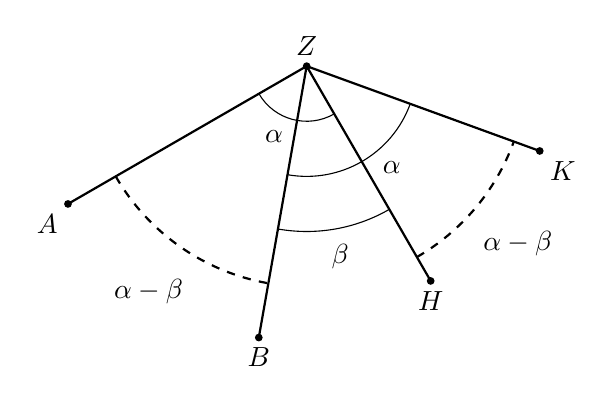
\begin{tikzpicture}[scale=.7]
\coordinate (Z) at (0,0);
\coordinate (A) at (-150:5cm);
\coordinate (B) at (-100:5cm);
\coordinate (H) at (-60:4.5cm);
\coordinate (K) at (-20:4.5cm);
\fill (Z) circle[radius=2pt];
\fill (A) circle[radius=2pt];
\fill (B) circle[radius=2pt];
\fill (H) circle[radius=2pt];
\fill (K) circle[radius=2pt];
\draw[thick] (A) node[below left] {$A$} -- (Z) node[above] {$Z$} -- (B) node[below] {$B$};
\draw[thick] (H) node[below] {$H$} -- (Z) -- (K) node[below right] {$K$};
\draw (-150:1cm) arc (-150:-60:1);
\draw (-100:2cm) arc (-100:-20:2);
\draw (-100:3cm) arc (-100:-60:3);
\draw[thick,dashed] (-150:4cm) arc (-150:-100:4);
\draw[thick,dashed] (-60:4cm) arc (-60:-20:4);
\node at (-115:1.4) {$\alpha$};
\node at (-50:2.4) {$\alpha$};
\node at (-80:3.5) {$\beta$};
\node at (-40:5) {$\alpha - \beta$};
\node at (-125:5) {$\alpha - \beta$};
\end{tikzpicture}
\vspace*{-10pt}
\end{center}

$\triangle ZAB\sim\triangle ZHK$ by SAS, since both are isosceles triangles and we have shown that they have the same vertex angle.

\vspace{-2ex}

\begin{center}
\begin{tikzpicture}[scale=.45]
\coordinate (Z) at (0,0);
\coordinate (A) at (-130:5cm);
\coordinate (B) at (-90:5cm);
\fill (Z) node[above left] {$Z$} circle[radius=4pt];
\fill (A) node[below left] {$A$} circle[radius=3pt];
\fill (B) node[below] {$B$} circle[radius=3pt];
\draw[name path=c1] (Z) circle[radius=5cm];
\draw[name path=c2] (Z) circle[radius=2.5cm];
\node at (2,5) {$c_1$};
\node at (2,2.5) {$c_2$};
\draw[thick] (A) -- node[below,yshift=-6pt] {$s$} (B);
\path[thick,dashed] (A) -- +(20:120pt) coordinate (H);
\fill (H) node[below] {$H$} circle[radius=3pt];
\path[thick,dashed] (B) -- +(60:120pt) coordinate (K);
\fill (K) node[right] {$K$} circle[radius=3pt];
\draw[thick] (Z) -- node[left,xshift=-2pt,yshift=-2pt] {$m$} (A);
\draw[thick] (Z) -- (B);
\draw[thick] (Z) -- (H);
\draw[thick] (Z) -- node[above] {$n$} (K);
\draw[thick] (H) -- node[below right] {$x$} (K);
\draw[thick,dashed] (A) -- (H);
\draw[thick,dashed] (B) -- (K);
\end{tikzpicture}
\end{center}

\vspace{-2ex}

Label $HK$ by $x$. Then:

\vspace{-2ex}

\erh{10pt}
\begin{equationarray*}{rcl}
\frac{m}{s} &=& \frac{n}{x}\\
x&=&\frac{n}{m}s\,.
\end{equationarray*}

%%%%%%%%%%%%%%%%%%%%%%%%%%%%%%%%%%%%%%%%%%%%%%%%%%%%%%%%%%%%%%%

\vspace{-2ex}


\section{Finding the intersection of two lines}\label{s.two-lines}

\textbf{Given two lines containing the line segments $AB,CD$, it is possible to construct their intersection using only a compass.}

$S$, the point of intersection of the two lines, lies on $AB$, because $\triangle CZS\cong \triangle C'ZS$ by SAS: $CZ=C'Z$, $\angle CZS=\angle C'ZS=90^\circ$ and $ZS$ is a common side. Therefore, $C'S=CS$ and similarly $D'S=DS$.


\begin{center}
\begin{tikzpicture}[scale=.8]
\coordinate (A) at (-4,0);
\coordinate (B) at (2,0);
\coordinate (C) at (-3,2);
\coordinate (D) at (1,-1);
\coordinate (Cp) at (-3,-2);
\coordinate (Dp) at (1,1);
\fill (A) node[below] {$A$} circle[radius=2pt];
\fill (B) node[below] {$B$} circle[radius=2pt];
\fill (C) node[above] {$C$} circle[radius=2pt];
\fill (D) node[below] {$D$} circle[radius=2pt];
\fill (Cp) node[below] {$C'$} circle[radius=2pt];
\fill (Dp) node[above] {$D'$} circle[radius=2pt];
\draw[name path=ab] ($(A)!1.3!(B)$) -- ($(B)!1.3!(A)$);
\draw[name path=cd] ($(C)!1.2!(D)$) -- ($(D)!1.1!(C)$);
\path [name intersections={of=ab and cd,by={S}}];
\fill (S) node[above] {$S$} circle[radius=2pt];
\draw (Cp) -- (Dp);
\draw[thick,dashed] (C) -- node[above left] {$c$} (Cp);
\draw[thick,dashed] (D) -- node[above right] {$d$} (Dp);
\path (C) -- node[right,xshift=2pt] {$x$} (S);
\path (S) -- node[left,near end,xshift=-2pt] {$e-x$} (D);
\node at (-1,-2.5) {\mbox{\boldmath $CD=C'D'=e$}};
\end{tikzpicture}
\end{center}

Label $x=CS, c=CC', d=DD',e=CD$. $\triangle CSC'\sim\triangle DSD'$ are similar so $\disfrac{x}{e-x} = \frac{c}{d}$. Solving the equation for $x$ gives $x=\disfrac{c}{c+d}e$.

If $C,D$ are on the same side of $AB$:
\begin{center}
\begin{tikzpicture}[scale=.8]
\coordinate (A) at (-4,0);
\coordinate (B) at (2,0);
\coordinate (C) at (-3,2);
\coordinate (D) at (-1,1);
\coordinate (Cp) at (-3,-2);
\coordinate (Dp) at (-1,-1);
\fill (A) node[below] {$A$} circle[radius=2pt];
\fill (B) node[below] {$B$} circle[radius=2pt];
\fill (C) node[above] {$C$} circle[radius=2pt];
\fill (D) node[above] {$D$} circle[radius=2pt];
\fill (Cp) node[below] {$C'$} circle[radius=2pt];
\fill (Dp) node[below] {$D'$} circle[radius=2pt];
\draw[name path=ab] ($(A)!1.3!(B)$) -- ($(B)!1.3!(A)$);
\draw[name path=cd] ($(C)!2.2!(D)$) -- ($(D)!1.1!(C)$);
\path [name intersections={of=ab and cd,by={S}}];
\fill (S) node[above] {$S$} circle[radius=2pt];
\draw (Cp) -- (S);
\draw[thick,dashed] (C) -- node[above left] {$c$} (Cp);
\draw[thick,dashed] (D) -- node[above right] {$d$} (Dp);
\path (C) -- node[above] {$e$} (D);
\path (Cp) -- node[below] {$e$} (Dp);
\path (D) -- node[above right,xshift=-4pt] {$x-e$} (S);
\path (Dp) -- node[below right,xshift=-4pt] {$x-e$} (S);
\node at (1,-2.5) {\mbox{\boldmath $CS=C'S=x$}};
\end{tikzpicture}
\end{center}
$\triangle CSC'\sim\triangle DSD'$ gives $\disfrac{x}{x-e}=\disfrac{c}{d}$. Solving for $x$ gives $x=\disfrac{c}{c-d}e$.

Construct the circles $c(C',d), c(D,e)$ and label their intersection by $H$. The sum of the line segments $CC',C'H$ is $c + d$. We have to show that $H$ is on the extension of $CC'$ so that $CH$ is a line segment of length $c+d$. ($CH = c - d$ in case $D$ is on the same side of $AB$ as $C$.) 

\vspace{-3ex}

\begin{center}
\begin{tikzpicture}[scale=.8]
\coordinate (A) at (-4,0);
\coordinate (B) at (2,0);
\coordinate (C) at (-3,2);
\coordinate (D) at (1,-1);
\coordinate (Cp) at (-3,-2);
\coordinate (Dp) at (1,1);
\fill (A) node[below left] {$A$} circle[radius=2pt];
\fill (B) node[below] {$B$} circle[radius=2pt];
\fill (C) node[above] {$C$} circle[radius=2pt];
\fill (D) node[below] {$D$} circle[radius=2pt];
\fill (Cp) node[left] {$C'$} circle[radius=2pt];
\fill (Dp) node[above] {$D'$} circle[radius=2pt];
\draw[name path=ab] ($(A)!1.3!(B)$) -- ($(B)!1.3!(A)$);
\draw[name path=cd] ($(C)!1.2!(D)$) -- ($(D)!1.1!(C)$);
\path [name intersections={of=ab and cd,by={S}}];
\fill (S) node[above,yshift=4pt] {$S$} circle[radius=2pt];
\draw (Cp) -- node[below right] {$e$} (Dp);
\path (C) -- node[above left] {$c$} (Cp);
\draw[thick,dashed] (D) -- node[above right] {$d$} (Dp);
\node at (3,-3) {\mbox{\boldmath $CD=C'D'=DH=e$}};
\draw[name path=circled] (D) let
  \p1 = ($ (D) - (C) $),
  \n2 = {veclen(\x1,\y1)}
in
  ++(130:\n2) arc (130:230:\n2);

\draw[name path=circlecp] (Cp) let
  \p1 = ($ (D) - (Dp) $),
  \n2 = {veclen(\x1,\y1)}
in
  ++(-180:\n2) arc (-180:0:\n2);
\path [name intersections={of=circled and circlecp,by={H}}];
\fill (H) node[below left] {$H$} circle[radius=2pt];
\draw[thick,dashed] ($(C)!1.2!(H)$) -- (C);
\draw (H) -- node[right] {$d$} (Cp);
\draw (D) -- node[right,xshift=14pt,yshift=8pt] {$e$} (H);
\end{tikzpicture}
\end{center}

\vspace{-3ex}

From the definition of $H$ as the intersection of $c(C',d)$,$c(D,e)$, we get $DH=e$, $C'H=d$, but $C'D' = e$, $D'D=d$, so the quadrilateral $C'D'DH$ is a parallelogram, since the lengths of both pairs of opposite sides are equal. By construction, the line segment $DD'$ is parallel to $CC'$, so $C'H$ is parallel to $DD'$ is also parallel to $CC'$. Since one of its end points is $C'$, it must be on the line containing $CC'$.

The lengths $c,d,e$ are given and we proved in Section~\ref{s.add-subtract} that a line segment of length $c+d$ can be construction and in Section~\ref{s.three} that a line segment of length $x=\disfrac{c}{c+d}e$ can be constructed. $S$ is the intersection of $c(C',x)$ and $c(C,x)$.

\begin{center}
\begin{tikzpicture}[scale=.8]
\coordinate (A) at (-4,0);
\coordinate (B) at (2,0);
\coordinate (C) at (-3,2);
\coordinate (D) at (1,-1);
\coordinate (Cp) at (-3,-2);
\coordinate (Dp) at (1,1);
\fill (A) node[below left] {$A$} circle[radius=2pt];
\fill (B) node[below] {$B$} circle[radius=2pt];
\fill (C) node[above] {$C$} circle[radius=2pt];
\fill (D) node[below] {$D$} circle[radius=2pt];
\fill (Cp) node[left] {$C'$} circle[radius=2pt];
\fill (Dp) node[above] {$D'$} circle[radius=2pt];
\draw[name path=ab] ($(A)!1.3!(B)$) -- ($(B)!1.3!(A)$);
\draw[name path=cd] ($(C)!1.2!(D)$) -- ($(D)!1.1!(C)$);
\path [name intersections={of=ab and cd,by={S}}];
\fill (S) node[above,yshift=4pt] {$S$} circle[radius=2pt];
\draw (Cp) -- (Dp);
\path (C) -- node[above,yshift=4pt] {$x$} (S);
\path (Cp) -- node[below,yshift=-4pt] {$x$} (S);
\path (C) -- node[above left] {$c$} (Cp);
\draw[thick,dashed] (D) -- node[above right] {$d$} (Dp);
\node at (2.5,-3) {\mbox{\boldmath $CD=C'D'=DH=e$}};
\draw[name path=circled] (C) let
  \p1 = ($ (S) - (C) $),
  \n2 = {veclen(\x1,\y1)}
in
  ++(-10:\n2) arc (-10:-100:\n2);

\draw[name path=circlecp] (Cp) let
  \p1 = ($ (S) - (C) $),
  \n2 = {veclen(\x1,\y1)}
in
  ++(100:\n2) arc (100:0:\n2);
\draw[thick,dashed] (Cp) -- (C);
\end{tikzpicture}
\end{center}

%%%%%%%%%%%%%%%%%%%%%%%%%%%%%%%%%%%%%%%%%%%%%%%%%%%%%%%%%%%%%%%

\section{Finding the intersection of a line and a circle}\label{s.line-circle}

\textbf{Given a circle $k=C(M,r)$ and a line $AB$, it is possible to construct their intersections using only a compass.}

Construct $M'$, be the reflection of $M$ about $AB$ and the circle $k'=c(M',r)$. The points of intersection of $k,k'$ are the points of intersection of the line $AB$ and the circle $k$.

\begin{center}
\begin{tikzpicture}[scale=.5]
\coordinate (A) at (-7,0);
\coordinate (B) at (8,0);
\coordinate (M) at (0,-2);
\coordinate (Mp) at (0,2);
\fill (A) node[below] {$A$} circle[radius=3pt];
\fill (B) node[below] {$B$} circle[radius=3pt];
\fill (M) node[below left] {$M$} circle[radius=3pt];
\fill (Mp) node[above left] {$M'$} circle[radius=2pt];
\draw[name path=c1] (M) circle[radius=3cm];
\draw[name path=c2] (Mp) circle[radius=3cm];
\draw[name path=ab] ($(A)!1.2!(B)$) -- ($(B)!1.2!(A)$);
\path [name intersections={of=c1 and c2,by={S1,S2}}];
\fill (S1) circle[radius=3pt];
\fill (S2) circle[radius=3pt];
\path[name path=radius1] (M) -- ++(15:4cm);
\path [name intersections={of=c1 and radius1,by={R1}}];
\draw[thick,dashed] (M) -- node[below] {$r$} (R1);
\path[name path=radius2] (Mp) -- ++(40:4cm);
\path [name intersections={of=c2 and radius2,by={R2}}];
\draw[thick,dashed] (Mp) -- node[above] {$r$} (R2);
\fill (R1) circle[radius=3pt];
\fill (R2) circle[radius=3pt];
\end{tikzpicture}
\end{center}

This construction cannot be done if $M$ is on the line $AB$. In this case, extend and shorten $AM$ by length $r$ as described in Section~\ref{s.add-subtract}. The end points of the extended and shortened segments are the intersections of $k$ with $AB$.


\begin{center}
\begin{tikzpicture}[scale=.5]
\coordinate (A) at (-7,0);
\coordinate (B) at (8,0);
\coordinate (M) at (0,0);
\fill (A) node[below] {$A$} circle[radius=3pt];
\fill (B) node[below] {$B$} circle[radius=3pt];
\fill (M) node[below left] {$M$} circle[radius=3pt];
\draw[name path=c1] (M) circle[radius=3cm];
\draw[name path=ab] ($(A)!1.2!(B)$) -- ($(B)!1.2!(A)$);
\path[name path=radius1] (M) -- ++(-30:4cm);
\path [name intersections={of=c1 and radius1,by={R1}}];
\draw[thick,dashed] (M) -- node[below] {$r$} (R1);
\path [name intersections={of=c1 and ab,by={S1,S2}}];
\fill (S1) node[above right] {$AM+r$} circle[radius=3pt];
\fill (S2) node[above left] {$AM-r$} circle[radius=3pt];
\fill (R1) circle[radius=3pt];
\end{tikzpicture}
\end{center}

